\documentclass[11pt,a4paper]{article}
\usepackage[margin=1in]{geometry}
\usepackage[T1]{fontenc}
\usepackage{lmodern}
\usepackage{microtype}
\usepackage{amsmath,amssymb,mathtools,bm}
\usepackage{booktabs,tabularx,array}
\usepackage{xcolor}
\usepackage{listings}
\usepackage{tikz}
\usetikzlibrary{arrows.meta,positioning,shapes.geometric,fit}
\usepackage[hidelinks]{hyperref}
\usepackage{enumitem}
\usepackage{caption}
\usepackage{float}
\setlist{nosep}
\definecolor{codebg}{RGB}{247,248,250}
\definecolor{codeblue}{RGB}{30,70,140}
\definecolor{codegreen}{RGB}{25,115,70}
\lstdefinestyle{python}{
  language=Python,
  basicstyle=\ttfamily\small,
  backgroundcolor=\color{codebg},
  keywordstyle=\color{codeblue}\bfseries,
  commentstyle=\color{codegreen},
  stringstyle=\color{red!65!black},
  numbers=left, numberstyle=\tiny\color{gray},
  breaklines=true, frame=single, rulecolor=\color{black!15},
  showstringspaces=false, columns=fullflexible
}
\title{Report 3: Grad-CAM Visualization, Interpretation, and Limitations for Audio}
\author{Technical Study Notes}
\date{\today}
\begin{document}
\maketitle
\tableofcontents
\newpage
\section{Purpose of the visualization}
The Grad-CAM computation produces one nonnegative value for each selected audio-token position. The visualization code maps this one-dimensional sequence onto the time axis of the input Mel-spectrogram and repeats it over all Mel-frequency bins. This makes the explanation easy to overlay on a conventional spectrogram, but the resulting image must be interpreted correctly: it expresses temporal importance only.

\section{The two arrays used in the overlay}
The input feature matrix is
\[
X\in\mathbb{R}^{M\times T_{\mathrm{in}}},
\]
where $M$ is the number of Mel bins and $T_{\mathrm{in}}$ is the number of time frames. The Grad-CAM vector from the audio tower is
\[
L\in\mathbb{R}^{T},
\]
where $T$ is the number of audio-token positions. These lengths need not be equal because the audio encoder can transform or downsample the time axis.

\section{Temporal interpolation}
The code reshapes the vector to $(1,1,T)$ and uses linear interpolation to obtain a vector of length $T_{\mathrm{in}}$:
\[
\widetilde{L}=\operatorname{Interp}_{\mathrm{linear}}
(L;\,T_{\mathrm{in}}).
\]
The operation estimates values between neighboring CAM samples. It is a display-alignment step, not a second neural-network inference and not a new attribution calculation.

The argument \texttt{align\_corners=False} controls the coordinate convention used by PyTorch's interpolation routine. It is commonly appropriate for resizing continuous signals. Nevertheless, proportional resizing is only an approximation to the true receptive-field alignment when the encoder uses nontrivial temporal strides, padding, chunking, or variable-length masking.

\section{Broadcasting over Mel frequency}
The code constructs
\[
H_{m,t}=\widetilde{L}_t,
\qquad
m=1,\ldots,M,\quad t=1,\ldots,T_{\mathrm{in}}.
\]
Equivalently, each time score is copied into every Mel bin. The matrix $H$ therefore has shape $(M,T_{\mathrm{in}})$, matching the spectrogram dimensions.

\begin{figure}[H]
\centering
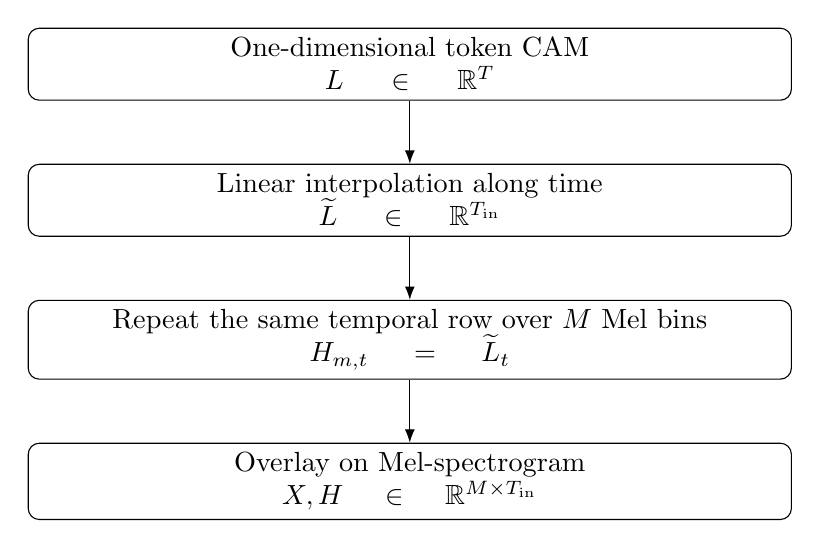
\begin{tikzpicture}[>=Latex, node distance=8mm,
box/.style={draw,rounded corners,align=center,minimum height=9mm,text width=0.78\linewidth}]
\node[box] (cam) {One-dimensional token CAM\\$L\in\mathbb{R}^{T}$};
\node[box,below=of cam] (resize) {Linear interpolation along time\\$\widetilde{L}\in\mathbb{R}^{T_{\mathrm{in}}}$};
\node[box,below=of resize] (rep) {Repeat the same temporal row over $M$ Mel bins\\$H_{m,t}=\widetilde{L}_t$};
\node[box,below=of rep] (overlay) {Overlay on Mel-spectrogram\\$X,H\in\mathbb{R}^{M\times T_{\mathrm{in}}}$};
\draw[->] (cam)--(resize); \draw[->] (resize)--(rep); \draw[->] (rep)--(overlay);
\end{tikzpicture}
\caption{The code converts a token-level temporal CAM into a spectrogram-sized display matrix.}
\end{figure}

This construction does not provide frequency localization. If a time frame is highlighted, all frequency bins at that frame are highlighted equally. Thus it is incorrect to conclude from this heatmap that the model specifically attended to a particular frequency band.

\section{Normalization}
The heatmap is divided by its maximum positive value when that maximum is greater than zero:
\[
H_{\mathrm{norm}}=
\begin{cases}
H/\max(H), & \max(H)>0,\\
H, & \max(H)\leq 0.
\end{cases}
\]
Because the CAM has already passed through ReLU, its entries should be nonnegative apart from numerical details. Normalization maps the maximum to one and preserves relative proportions within the same example.

\subsection{What normalization does not mean}
A normalized score of $1$ means only that the location is the maximum in that displayed map. It does not mean 100 percent probability, 100 percent contribution, or a calibrated measure of clinical importance. Comparisons across recordings require care because each map may have been independently normalized.

\section{Interpreting positive Grad-CAM}
The target score is
\[
s=z_{\mathrm{PD}}-z_{\mathrm{HC}}.
\]
The Grad-CAM map is constructed from gradients of this score. A bright region therefore indicates a time region with a relatively large positive Grad-CAM value under the chosen layer and averaging procedure. It can be described as a region whose learned representation is associated with positive support for the PD-versus-HC logit contrast.

It should not be described as proof that the region contains a disease-specific acoustic marker. Gradients are local sensitivities, and the network may use correlated, spurious, or dataset-specific cues. A visualization is an explanation of model behavior, not a clinical validation.

\section{Positive and negative evidence}
The ReLU operation discards negative values:
\[
L_t=\max(0,C_t).
\]
This is standard for positive Grad-CAM maps. It means that the displayed map does not show locations whose weighted contribution is negative for the selected score. If the research question includes both evidence for PD and evidence against PD, retain and inspect the signed pre-ReLU quantity
\[
C_t=\sum_k\alpha_k A_{t,k}
\]
or create a separate visualization for negative values. Such alternatives should be clearly distinguished from conventional positive Grad-CAM.

\section{Comparison with Integrated Gradients}
Integrated Gradients (IG) is a different attribution method. It attributes the output to input features by integrating gradients along a path from a baseline input $X'$ to the actual input $X$:
\[
\operatorname{IG}_i(X)=
(X_i-X'_i)\int_0^1
\frac{\partial F(X'+\lambda(X-X'))}{\partial X_i}
\,d\lambda.
\]
Here $F$ is the scalar target score and $i$ indexes an input feature, such as a time-frequency cell in the Mel-spectrogram. In practice, the integral is approximated using a finite number of interpolation steps.

\begin{center}
\begin{tabularx}{\linewidth}{lXX}
\toprule
\textbf{Aspect} & \textbf{Grad-CAM used here} & \textbf{Integrated Gradients}\\
\midrule
Attribution basis & Internal layer activations and gradients & Input gradients integrated along a baseline path\\
Baseline required & No & Yes\\
Natural output here & One value per audio-token position & Potentially one value per input time-frequency cell\\
Resolution & Layer-dependent and coarse & Input-feature resolution, subject to preprocessing\\
Main design choice & Target layer and target score & Baseline, target score, and integration steps\\
Interpretation & Positive evidence in a selected representation & Attribution relative to the chosen baseline\\
\bottomrule
\end{tabularx}
\end{center}

Neither method is automatically more accurate. They answer related but different questions. Grad-CAM is useful for a compact temporal overview. Input-level IG can provide frequency-resolved attribution if gradients are computed with respect to the two-dimensional input features and the model supports that differentiable path.

\section{Why the current map is not frequency-resolved}
The current code averages gradients over token positions, weights hidden features, sums over the hidden dimension, and obtains a scalar per token. At no stage does it preserve an explicit Mel-frequency axis. The Mel bins are introduced again only when the temporal vector is repeated to create a display matrix.

Therefore, the resulting heatmap is not a two-dimensional Grad-CAM in the time-frequency sense. It is a one-dimensional temporal attribution expanded to fit a two-dimensional plot.

\section{Practical validation recommendations}
\begin{enumerate}
\item \textbf{Inspect shapes.} Print the activation, gradient, CAM, resized CAM, and input-feature shapes. Verify that the expected dimensions are used.
\item \textbf{Inspect layer output structure.} Check whether the layer returns a tensor or tuple and confirm that the selected tuple element is the hidden-state tensor.
\item \textbf{Check gradient existence.} Verify that \texttt{activation.grad} is not \texttt{None} after \texttt{score.backward()}.
\item \textbf{Check score semantics.} Confirm that the selected PD and HC token IDs and final sequence position represent the intended classification contrast.
\item \textbf{Check temporal alignment.} Confirm whether the audio tower's token positions map uniformly to the input time axis. Account for padding, stride, or chunking if necessary.
\item \textbf{Avoid overclaiming.} Describe the output as temporal model attribution, not a frequency-specific explanation or clinical biomarker.
\item \textbf{Compare methods.} Where appropriate, compare Grad-CAM with input-level attribution such as Integrated Gradients and assess whether salient regions are stable.
\item \textbf{Test robustness.} Examine multiple recordings, perturbations, and model seeds. A single heatmap is not sufficient evidence of reliable explanation.
\end{enumerate}

\section{Common interpretation errors}
\begin{description}
\item[Error: The brightest point is a 100\% contribution.] The map is normalized for display; it is not a probability or percentage.
\item[Error: The map identifies an important frequency band.] The code repeats each temporal value across all Mel bins and therefore has no frequency discrimination.
\item[Error: The hook computes the gradient.] The hook captures the activation and calls \texttt{retain\_grad()}; \texttt{backward()} computes the gradient later.
\item[Error: \texttt{output[0]} means the first layer.] It means the first element of a tuple returned by the selected layer. The last layer is selected separately by \texttt{layers[-1]}.
\item[Error: A positive map proves causality.] It indicates positive Grad-CAM response for a chosen score and layer, not a causal clinical mechanism.
\end{description}

\section{Conclusion}
The visualization pipeline transforms the final audio-layer Grad-CAM into a spectrogram-sized temporal overlay. Linear interpolation aligns the number of time samples, row repetition broadcasts each time score across Mel bins, and maximum normalization makes the map convenient to display. The result is useful as a temporal overview of the model's PD-versus-HC score, but it must not be interpreted as frequency-specific attribution. Integrated Gradients or another input-level method can complement it when time-frequency localization is required.

\end{document}
